% A skeleton file for producing Computer Engineering reports
% https://kgcoe-git.rit.edu/jgm6496/KGCOEReport_template

\documentclass[CMPE]{../KGCOEReport}

% The following should be changed to represent your personal information
\newcommand{\classCode}{EEEE 380}  % 4 char code with number
\newcommand{\name}{Andrei Tumbar}
\newcommand{\LabSectionNum}{1}
\newcommand{\LabInstructor}{Dr.\ Moon}
\newcommand{\TAs}{Karen Chen}
\newcommand{\exerciseNumber}{4}
\newcommand{\exerciseDescription}{CMOS Combinational Logic}

\usepackage{tikz}
\usepackage{circuitikz}
\usepackage{multirow}
\usepackage{titlesec}
\usepackage{float}
\usepackage{lmodern}
\usepackage{siunitx}
\usepackage{subcaption}
\usepackage{graphicx}
\usepackage[usestackEOL]{stackengine}
\usepackage{scalerel}
\usepackage[T1]{fontenc}
\usepackage{amsmath}


\def\code#1{\texttt{#1}}

\begin{document}
    \maketitle
    \section*{Abstract}

    In this exercise, the behaviour of a three input NAND
    gate was investigated. A voltage sweep of the three inputs
    were swept to show the inverter behaviour that can be seen
    from the NAND gate. All of the inputs of the NAND3 gate
    were tested to show the proper opertion of the NAND gate. \\

    \section*{NAND3 Input Sweep}
    
    The pull-down network of the NAND3 gate will experience body effect.
    The three NMOS transistors are placed in series meaning two of the
    devices will experience body effect. The circuit was simulated with and
    without body effect at $V_{50\%}$ by setting $\gamma$ to $0$ and $0.2$.

	\begin{table}[h!]
		\renewcommand{\arraystretch}{1.3}
		\setlength{\tabcolsep}{12pt}
		\caption{$V_{50\%}$ with and without body effect.}
		\begin{center}
		    \begin{tabular}{|c|c|c|c|c|}\hline
		    & $V_{out}$ & X & Y & I\\\hline
		    No body & 1.70995 & 0.359252 & 0.155978 & 0.0036125 \\\hline
		    Body    & 1.85866 & 0.33856 & 0.146403 & 0.00341177 \\\hline
		    \end{tabular}
		\end{center}
		\label{tab:cmos}
	\end{table}

	Looking at the results, it makes sense that the voltage drop
	over the NMOS transistors experiencing body effect is larger
	than without body effect. This is why the voltage at the $X$ and
	$Y$ nodes is lower as the top NMOS transistor was the largest
	voltage drop.\\

     A voltage input sweep of the NAND3 gate was performed
     to show the effective inverter behaviour of the gate.
     
     \begin{figure}[h!]
     	\centering
       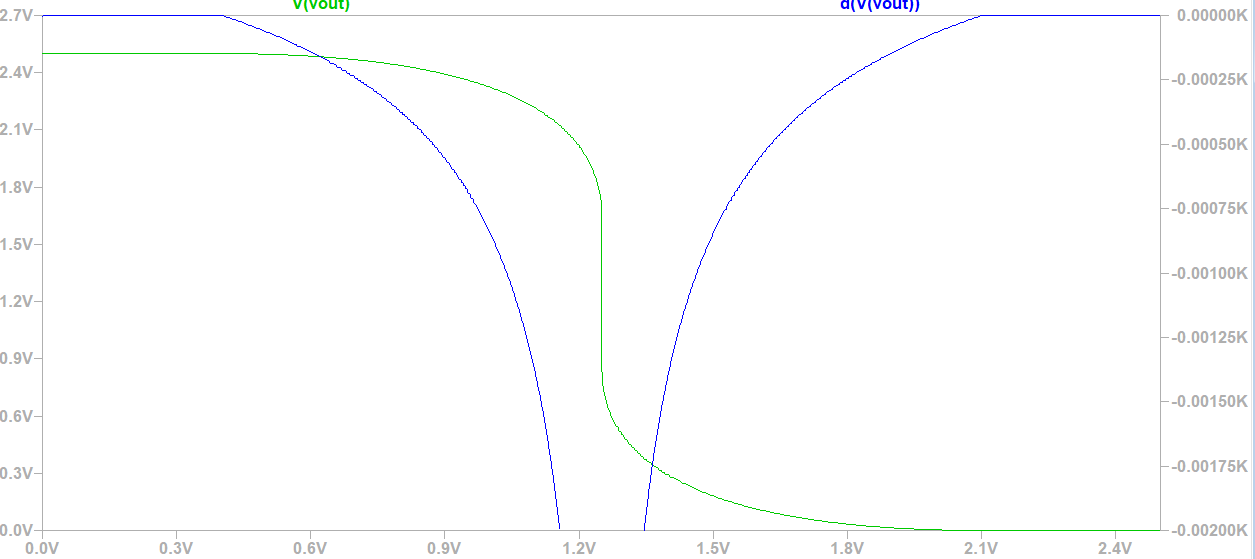
\includegraphics[width=5.5in]{img/nand_sweep.png}
       \caption{RTC NAND3 input sweep}
       \label{fig:nand_sweep}
	 \end{figure}

	Figure \ref{fig:nand_sweep} shows the expected VTC curve that
	would be seen from an inverter as all of the inputs are hooked
	together. Because the NAND gate was designed to have equal noise
	margins ($NMH = NML$), the VTC is semetrical when looking on
	either side of the $V_{th}$. This also shows that the power of the
	pull-up network is equal to the power of the pull-down network.\\

	\section*{NAND Functionality}
	
	To test the NAND gate, a set of all the input combinations were simulated
	in PSPICE. The NAND3 gate should output high in all cases expect when all
	the inputs are high.

	\begin{figure}[h!]
     	\centering
       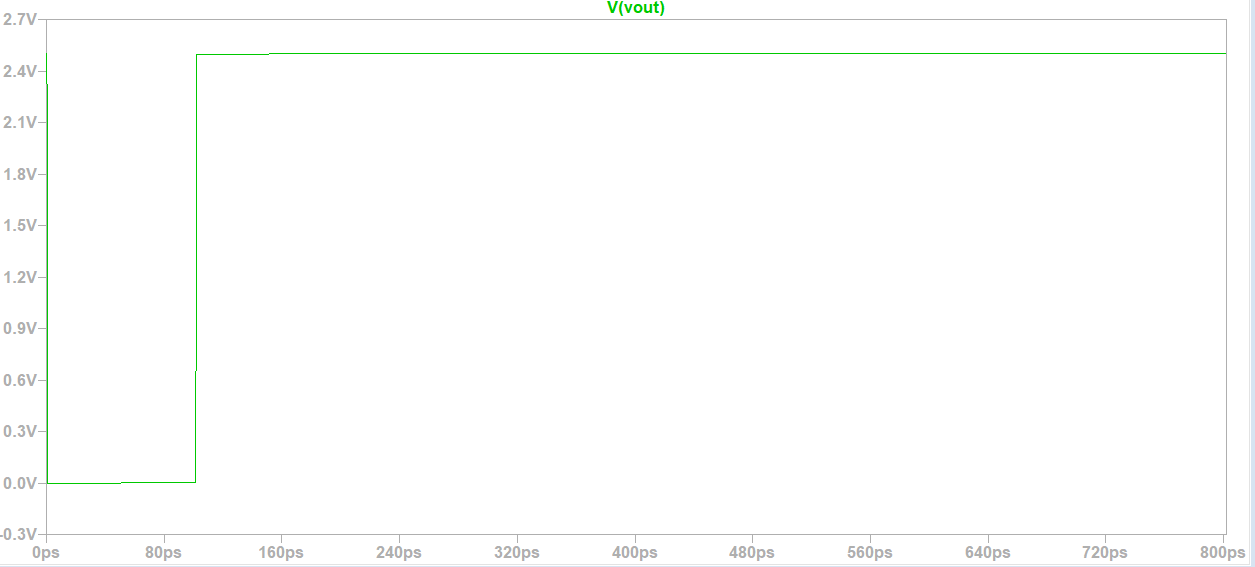
\includegraphics[width=5.5in]{img/nand_pulse.png}
       \caption{NAND3 gate output for all input combinations}
       \label{fig:nand_pulse}
	 \end{figure}

	The output of the NAND3 gate is as expected. The first input combination
	is when $A=1$, $B=1$, $C=1$ and the output is low which is expected.
	All other input combinations are high which is also expected. 

	\section*{Conclusion}
	This laboratory exercise looked at the logical properties of the
	NAND3 gate. The response of the NAND3 gate with and without body
	effect was investigated. Next, an input sweep for all three inputs
	was performed to show that the noise margins and PUN/PDN strengths
	were calculated correctly. Finally, the logical behaviour of the gate
	was tested by running all of the input combinations. The expected
	behaviour of the NAND3 gate was observed in all of the different tests
	performed.

\end{document}
